% !TEX program = xelatex
\documentclass[11pt]{article}
\usepackage{balance,graphics,fontspec,setspace,titling,fmtcount,graphicx}
\usepackage{natbib,sidecap,subcaption,hyperref,setspace}

\usepackage[page,toc]{appendix}
\usepackage[margin=1in]{geometry}
\usepackage[inline]{enumitem}
\usepackage[tiny,compact]{titlesec}

\setcitestyle{authoryear, open={(},close={)}}

% \linespread{2}

% \doublespace
\setmainfont[
Ligatures=TeX,
Extension=.otf,
UprightFont= *-regular,
BoldFont=*-bold,
ItalicFont=*-italic,
BoldItalicFont=*-bolditalic]{texgyretermes}
\setmonofont{Source Code Pro}



\setlength{\parskip}{.4em}
\setlength{\parindent}{0em}
\newcounter{countitems}
\newcounter{nextitemizecount}
\newcommand{\setupcountitems}{%
  \stepcounter{nextitemizecount}%
  \setcounter{countitems}{0}%
  \preto\item{\stepcounter{countitems}}%
}
\makeatletter
\newcommand{\computecountitems}{%
  \edef\@currentlabel{\number\c@countitems}%
  \label{countitems@\number\numexpr\value{nextitemizecount}-1\relax}%
}
\newcommand{\nextitemizecount}{%
  \getrefnumber{countitems@\number\c@nextitemizecount}%
}
\makeatother
\AtBeginEnvironment{inlinelist}{\setupcountitems}
\AtEndEnvironment{inlinelist}{\computecountitems}
\AtBeginEnvironment{enumerate}{\setupcountitems}
\AtEndEnvironment{enumerate}{\computecountitems}
\AtBeginEnvironment{itemize}{\setupcountitems}
\AtEndEnvironment{itemize}{\computecountitems}


\titlespacing*{\section}
{0pt}{0pt}{0pt}
\titleformat*{\subsection}{\it}

\setlist[itemize]{itemsep=0pt,topsep=0pt,parsep=0pt}
\setenumerate{itemsep=0pt,topsep=0pt,parsep=0pt}
\newcommand{\sectitle}[1]{\textit{#1}}

\newlist{inlinelist}{enumerate*}{1}
\setlist*[inlinelist,1]{
  label=\arabic*),
}


\title{Worker Experience and Collective Action in an Online Piecework Economy}
\author{
Michael Bernstein\\
Computer Science, Stanford University
\and
Margaret Levi\\
Political Science and CASBS, Stanford University
}
\begin{document}
\begin{titlingpage}
  \maketitle
\end{titlingpage}

\pagebreak
\begin{abstract}
The digital gig economy has led to a resurgence of piecework.
Without shared factories and water coolers,
how do digital pieceworkers coordinate,
build solidarity,
and take collective action?
We will engage in fieldwork to understand
how digital pieceworkers engage in collective behavior
to better their work conditions.
Ethnographic fieldwork will take place on worker forums,
and in a cooperatively-owned labor market.
Our goal is to understand the drivers and inhibitors of collective behavior in online work.
Results will impact the design and infrastructure of the growing gig economy,
and the policies necessary for collective action by workers to succeed online.
\end{abstract}



\section{Introduction}
Generally, piecework disempowers workers and empowers employers.
Piecework drives employees to work faster and longer,
affording them little control over their working conditions.
For most of its history, piecework offered no
  benefits,
  occupational health and safety,
  or social insurance.
When piecework combines with the routinization of jobs,
workers become interchangeable and deindividuated,
another form of disempowerment.
Piecework was the dominant form of payment system during the industrial era,
starting with agriculture and home production but quickly moving into factories.
At the turn of the 20th century in the U.S.,
campaigns for workers' rights had yielded regulations on conditions.
By the late 20th century, however, piecework was associated primarily with migrant labor and sweatshops.

Today, with the growth of the digital gig economy, piecework is reemerging in new forms.
Networked computational infrastructure is now mediating each unit of work and worker.
Uber's taxi drivers are paid per ride and assigned jobs by an algorithm
\citep{uberAlgorithm,hall2015analysis}.
Information workers
--- such as those on Amazon Mechanical Turk (AMT) and Upwork ---
are paid per task, performing vast quantities of data and administrative work
\citep{martin2014being}.
Increasing numbers of workers make money through one--off tasks like
  housecleaning
  and food delivery,
all mediated by online platforms.
Current legal and policy frameworks classify these workers as
\textit{independent contractors},
precluding them from accessing employee benefits and job security associated with employment.

Digital piecework reframes many of the historical dynamics.
In one sense, it is a return to piecework in the home,
where the worker controlled the hours worked.
Seeing few alternatives,
home pieceworkers found themselves deciding whether to work in dangerous conditions or to starve.
However, in another sense,
online pieceworkers make this scenario quite different,
prizing the flexibility and autonomy afforded by their platforms
\citep{martin2014being}.
Many view themselves as masters of their own fate, free to enter and leave the workforce at will and without repercussion.

These trends in labor are not new,
but have accelerated with the growth in digital mediation.
With relatively scant research on the magnitude of this digitally mediated,
transient labor force,
and lack of consensus regarding the exact boundaries describing this mode of labor,
estimating the true scale of the gig economy has proven difficult.
Nevertheless,
TIME's most recent poll of so--called
``sharing economy'' workers led them to conclude that
as many as forty five million Americans have offered goods or services through these marketplaces
\citep{sharingEconomyPoll}.
With nearly 20 percent of jobs in the United States that could be potentially sent
``down the wire''
\citep{blinder2006offshoring}
via services such as this,
the gig economy's rapid growth and large potential workforce necessitates a focused research and policy agenda.

Especially important,
we as yet have limited knowledge of how
collectives of online pieceworkers are adapting to contemporary labor markets.
Furthermore, we do not know how workers are engaging in coordinated and cooperative reactions.
Are their efforts similar to historical efforts for offline pieceworkers,
such as unions and worker cooperatives?
Or do the affordances of the online world result in different outcomes?

How do workers react, and create collective counterbalances,
to the digital piecework economy?
On one hand, studies of online communities predict that
workers online will face greater challenges because
trust is more difficult to build in digitally mediated environments
\citep{successfulOnlineCommunities,kollock2005managing,cook2005cooperation}.
Without
  factory floors,
  water coolers, and
  shared neighborhoods
\citep{waterCooler},
how do workers coordinate and build solidarity?
On the other hand,
online forums may make it easier for workers to
  share information and
  coordinate strategies with relative anonymity,
and successful collective efforts
such as Wikipedia
suggest that online environments may support collectives
that could not have succeeded as readily offline.

We propose grounded ethnographic fieldwork to understand the forces shaping informal and formal worker reactions to the online piecework economy.
We will perform a coupled analysis of worker behavior in
\begin{inlinelist}
  \item the current sociotechnical ecosystem and in 
  \item emerging platforms for worker cooperativism and collective action
\end{inlinelist}
First, through a year of fieldwork on
  major Mechanical Turk (data entry) platforms and forums, and
  on gig economy platforms such as Uber (driving) and
  Handy (domestic work),
we will investigate the techniques that workers utilize
to manage their work environments and job opportunities.
We will seek to understand the challenges they face when
balancing an identity of being self--employed with
          an identity of being a pieceworker for a privately--owned labor platform.
Second, we will engage with workers using
recently developed platforms for collective action on Mechanical Turk
for forming worker cooperatives in the gig economy
to understand how formal efforts succeed and fail.

Our team is uniquely qualified to pursue this opportunity.
Levi has years of experience studying
  labor,
  collectives, and
  unions.
She is pairing with Bernstein,
a computer scientist who studies online labor platforms and collective action.
Bernstein, alongside Ph.D.
students Salehi and Alkhatib,
created the first platform for collective action efforts amongst digital pieceworkers,
focused on the Amazon Mechanical Turk platform.
This effort has galvanized hundreds of workers and
resulted in outcomes including public media campaigns and
the creation of ethical work guidelines for Mechanical Turk employers.

This work carries policy implications for the emerging,
and as yet largely unregulated, gig economy.
What affordances and protections do workers need in order to unionize,
or gather, effectively?
What protections should platforms be required to provide to their workers?
What support is necessary for people who work on multiple platforms,
frequently moving between different employers?


\section{Related Work}


The form of work that we propose to study has ties to previously--studied communities,
but various features make the context and framing of this field site unique.
Myriad lenses can be used to appreciate the qualities of gig work; we will explore
\nextitemizecount{}
of them here:
\begin{inlinelist}
  \item Taylorism and the rise of the routinization of work, and
  \item piecework, and the parallels between historical piecework and its contemporary gig work.
\end{inlinelist}

The parallels between Taylorism and gig work on digitally mediated labor markets
--- especially markets for information work such as AMT ---
are striking, perhaps for unsurprising reasons.
Whereas these markets advertise the work as
``\textit{artificial} artificial intelligence'',
the reality, as
\citeauthor{turkopticon}
point out,
belies the true nature of the platform and dehumanizes the workers behind the scenes
\citep{turkopticon}.
This distancing from the human features of AMT promotes a framing of work that is
\begin{inlinelist}
  \item compartmentalizable (wherein tasks can be broken into smaller components),
  \item decontextualizable (describing the alienation of work about which
  \citeauthor{marx2012economic}
  writes
  \citep{marx2012economic}), and
  \item readily testable (that is, provably true or untrue).
\end{inlinelist}

The relationship between piecework and gig work is important to appreciate, both
to frame our understanding of emergent trends in labor
as well as
to inform our theories for worker empowerment later.
Through this lens, we find the work of
\citeauthor{riisOtherSideLives}
and others informative
\citep{riisOtherSideLives,gringeri1994getting,herzog1980hand}.
The study of piecework represents not only a historical insight,
but a global one as well;
\citeauthor{shaheed1983invisible}
describe the role of piecework among women in Lahore,
and
\citeauthor{hahn1996feminization}
explores the gendered nature of piecework in India
\citep{shaheed1983invisible,hahn1996feminization}.

Considering the empowerment of workers in broader contexts,
we find a substantial body of literature which informs our theoretical framing as well.
In framing this body of research,
we identify \nextitemizecount{} themes:
\begin{inlinelist}
  \item the collaborative nature of gig work, namely on Amazon Mechanical Turk (AMT),
  \item efforts toward collective action and the challenges that stymie these groups, and
  \item more historical perspectives on collective action and the challenges that problematize it.
\end{inlinelist}

To understand sustained collective action,
\citet{russell1982collective}
calls for an
``anthropological investigation of minute interrelationships''
and the institutions in which those relationships occur
\citep[see also
\citet{hirschman1970exit,ostrom1990governing,polletta2002freedom}
]{russell1982collective}.
% [Hardin,
% 1982,
% also see Hirschman [1970]; Ostrom [1990]; Polletta [2002]].
Digital ethnographic fieldwork has detailed how workers gather in virtual spaces
--- such as forums and chat rooms ---
to
  discuss their work,
  share best practices, and
  manage their relationship with employers
\citep{martin2014being}.
The crowd of independent,
dispersed workers is in fact a collaborative network
\citep{crowdcollab}.
While this research has established that
  workers share information and build social connections,
it is not clear how they may engage in more complicated forms of collective action.

Research on online collective action explores
the social dynamics involved when groups aggregate their efforts online to push a cause.
In a setting where people can cheaply communicate with like--minded individuals,
collectives can overcome many of the challenges that stymie offline groups
\citep{earl2011digitally}.
But they still face free rider problems
\citep{olsonlogic},
the choice of exit or voice
\citep{hirschman1970exit},
and newcomers perceptions of favoritism towards veterans
\citep{polletta2002freedom}.

For example,
digitally mediated communities
such as Wikipedia
confront accusations of elite ``gatekeepers'',
paralleling the perceptions of oligarchism within allegedly egalitarian and
participatory governance systems
\citep{keegan2010egalitarians}.
We can learn from the experiments attempting to make sites of peer production
like Wikipedia
more inclusive and transparent.
Further,
a wealth of literature identifies both
  worthwhile practices and
  pitfalls that might endanger similar organizations
\citep{weber2004success,mockus2002two}.

Work to date addresses
--- but only to a limited extent ---
the limits and possibilities of cooperation among online workers.
Our research enables us to go into far greater depth on these questions
than previous studies have been able to do.
The combination of field work,
comparisons of different kinds of jobs and work organization,
and experiments with platforms will allow us to identify more specific
  mechanisms,
  processes, and
  contexts
that facilitate (or block) varieties of collective action.


\section{Prior work by the PIs}

Michael Bernstein is an Assistant Professor at Stanford and a computer scientist who
  designs,
  engineers, and
  studies
online work.
He is the recipient of
  a Sloan Research Fellowship,
  NSF CAREER grant, and
  George M. Sprowls Award for best doctoral thesis in Computer Science at MIT.
His group's research has received Best Paper awards and nominations at premier venues in
human--computer interaction.
Recently, his group, led by Ph.D. students
  Niloufar Salehi and
  Ali Alkhatib,
created the We Are Dynamo platform,
which enabled workers on Amazon Mechanical Turk to take collective action.
Hundreds of workers have participated in the site,
leading to two major campaigns:
\begin{inlinelist}
  \item The creation of worker--authored ethical research guidelines
  for research on Amazon Mechanical Turk at \url{http://guidelines.wearedynamo.org};
  \item A public media campaign of open letters to
  Amazon CEO Jeff Bezos
  to advocate for workers' perspectives on labor issues with Mechanical Turk.
\end{inlinelist}
Subsequent to this effort, several requests
(e.g., reinstatement of some workers accounts)
were implemented by Amazon.

Margaret Levi is a comparative political economist,
whose work focuses on
  government and governance,
  cooperation and trust,
  citizenship, and
  labor.
From 1994--2004,
she was the co--director with
  Russell Hardin and
  Karen Cook
of the RSF project on trust,
and she remains co--general editor of the RSF Trust series.
She co--authored one book in the series and edited or co--edited several others.
Levi has also written three books that explore the relationships of
  workers with their
    governments,
    employers, and
    unions.
In particular,
she has investigated the conditions under which
\begin{inlinelist}
  \item workers overcome collective action problems to organize unions
    in the United States and
    around the world,
  \item gain recognition for their unions and
    collective bargaining rights, and
  \item develop an expanded community of fate
  that takes into account distant others and
  on whose behalf the workers are willing to take costly actions.
\end{inlinelist}


\section{Research Proposal}
This research calls for cross--cultural analysis,
first exploring the communities and support structures which emerge in piecework markets run by external managers,
and subsequently their counterpart organizations and structures which form in cooperatively--run piecework labor markets.
Our work will explore two fundamentally different types of labor markets: labor markets run by external managers
(e.g. Uber, Lyft, Amazon Mechanical Turk, etc\dots),
and labor markets run cooperatively
(i.e. owned and managed by the system's workers themselves).

\subsection{Investigating Current Coping Strategies}\label{ethnography}
The first study will consist of ethnographic fieldwork studying workers in modern piecework labor markets
--- e.g., Mechanical Turk, Uber, and Handy ---
to understand how social coping strategies emerge among workers.
How do workers air their grievances?
How do they come together to push for change?
How have they adapted to the working conditions of these digital hiring halls?

\citet{uberAlgorithm}
and others have identified a number of ways that workers
  navigate and even
  subvert the intent of system--designers.
These patterns of behavior elude
  algorithmic tracking and
  measurement
because they deliberately avoid the \textit{a priori} assumptions made by the designers of systems,
who attempt to structure these sites of work in ways to incentivize preferred behavior.
Identifying and understanding the details of this behavior thus begins with a
  qualitative,
  ethnographic
endeavor.

We will perform fieldwork with digital pieceworkers.
To understand their breadth of experience,
we will sample roughly fifty workers from information work
(for example, Mechanical Turk and CrowdFlower),
and another
fifty workers in the ``sharing economy''
(including
  Uber,
  Lyft, and
  AirBnB),
and fifty in gig work
(namely Handy and TaskRabbit).
Given
  existing relationships and
  reputations
as credible researchers in communities of \textit{Turkers},
we can recruit participants through known existing channels.
In the cases of platforms such as
  Uber,
  AirBnB, and
  Handy,
we can recruit workers for nominally legitimate work
(for example, requesting that a driver drives for 15 minutes to a previously selected destination)
and invite them to participate in our interview.

Through a combination of
  semi--structured interviews,
  surveys, and
  grounded analysis of worker forums,
we will seek to better understand workers' relationships
  with the externally--managed platforms,
  with their clients, and
  with each other.
Our questions will include
contextualizing questions asking
  how long the worker has worked in that platform and
  what sort of work they engaged in before they worked on that platform.
Excluding questions and topics of discussion that emerge from these prompts,
we will ask workers
  what parts of their platforms and styles of work they enjoy and
  what parts they find frustrating,
which will segue into further questions about
whether and how people work around the system when it fails to do what they wish.

Further,
we will investigate how workers rely on each other
despite being distributed and never meeting face--to--face,
and how they collectively act to counter the directives and desires of their employers.
We seek to uncover
  how norms emerge,
  how workers discover one another, and
  how techniques for subverting systems are
discovered and
communicated across these geographically dispersed,
and often seemingly disconnected,
communities of workers.

These insights will inform the broader question of
how collective action among digitally mediated communities works,
and in particular expose how members of networked communities
--- typically considered too decentralized and diffuse to allow such phenomena to occur ---
successfully engage in collective behavior.
These behaviors often work
to expose and
capitalize on unexpected flaws in employers' algorithms and policies
--- for example, how Uber drivers will rapidly toggle their availability on and off
in order to contravene the Uber availability algorithm,
which would otherwise automatically grow the geographic radius in which a driver must pick up a ride if they have not found a ride recently
\citep{uberAlgorithm}.

\subsection{Understanding Emerging Cooperativism}\label{Alia}
Armed with a better understanding of workers' needs and collective behaviors,
we next seek to study worker behavior in a platform that better represents workers' needs.
However, solutions that exist for traditional, non--gig workers
--- especially labor unions ---
face resistance from workers in the gig economy
\citep{martin2014being,dynamo}.
This distaste may be due to a general decline in public opinion of unions.
However,
the traditional mechanics of a labor union are also a poor match: challenging issues include managing the benefits and proportional representation of workers whose contracts may last only minutes or hours,
enforcing collective decisions on a decentralized network of workers,
and establishing trust between workers who may never meet face--to--face.
In our early fieldwork, for example,
a worker on Amazon Mechanical Turk stated:
``If by `union' you mean a `labor union',
I would not feel comfortable taking part.
It runs against my grain because I am an individualist.
[\dots] I consider myself self--employed\dots~not working for anyone in particular''
\citep{dynamo}.

Given these constraints,
we seek to understand:
what model would give workers more power in an online gig--economy platform
while still enabling a market to emerge and function?
To explore one such alternative,
we are collaborating with the National Domestic Workers Alliance's innovation arm,
the Fair Care Labs,
on tools for online pieceworkers to collectively manage and govern their own labor markets.
While the literature in
social computing design and
crowdsourcing
already features many tools for successful decentralized collaborations
(e.g., Wikipedia),
and collective action movements
(e.g., change.org),
templates and guidelines for
sustained collective action and
governance online in high--stakes situations
that affect workers' livelihoods are rare.
Such efforts tend to swell quickly,
but soon find themselves embroiled as they struggle to satisfy myriad stakeholders.
Our goal is to introduce design mechanisms
to enable collectives of gig workers to form,
debate policy,
and implement their decisions over a long period of time.

In collaboration with
the National Domestic Workers Alliance's innovation arm
--- the Fair Care Labs ---
we are designing and launching a cooperative gig labor market for
domestic workers (house cleaners).
This cooperative labor market, ``Alia'',
is designed for domestic workers in the California Bay Area.
However, our interest
--- and the Fair Care Labs' ---
is to generalize its insights to other workers and industries.
While the driving domain is already crowded with services such as Lyft and Uber,
domestic work is a more ideal area to launch a research prototype.
In addition,
the NDWA Fair Care Labs' support and network will help us gain rapid traction.
The web and mobile application,
Alia, enables the basic affordances of ``gig'' work for domestic work
--- rapid scheduling of any available worker in the network
(see figure~\ref{fig:Alia} on page~\pageref{fig:Alia}).

\begin{figure}
\centering
    \begin{subfigure}[b]{0.3\textwidth}
        
\includegraphics[width=\textwidth]{figures/1.png}
        % \caption{A gull}
        \label{fig:sched}
    \end{subfigure}
    ~ %add desired spacing between images, e. g. ~, \quad, \qquad, \hfill etc. 
      %(or a blank line to force the subfigure onto a new line)
    \begin{subfigure}[b]{0.3\textwidth}
        
\includegraphics[width=\textwidth]{figures/2.png}
        % \caption{A tiger}
        \label{fig:confirm}
    \end{subfigure}
    ~ %add desired spacing between images, e. g. ~, \quad, \qquad, \hfill etc. 
    %(or a blank line to force the subfigure onto a new line)
    \begin{subfigure}[b]{0.3\textwidth}
        
\includegraphics[width=\textwidth]{figures/3.png}
        % \caption{A mouse}
        \label{fig:profile}
    \end{subfigure}
    \caption{Alia, our prototype cooperative platform for collective governance in a gig marketplace.
             Alia is targeted as a marketplace for domestic workers to do rapid online bookings.
             Its main research goal is to examine affordances for
             collective decision--making and
             governance in a cooperative marketplace.}\label{fig:Alia}
\end{figure}
% \begin{SCfigure}
% \centering
% \caption{}
% 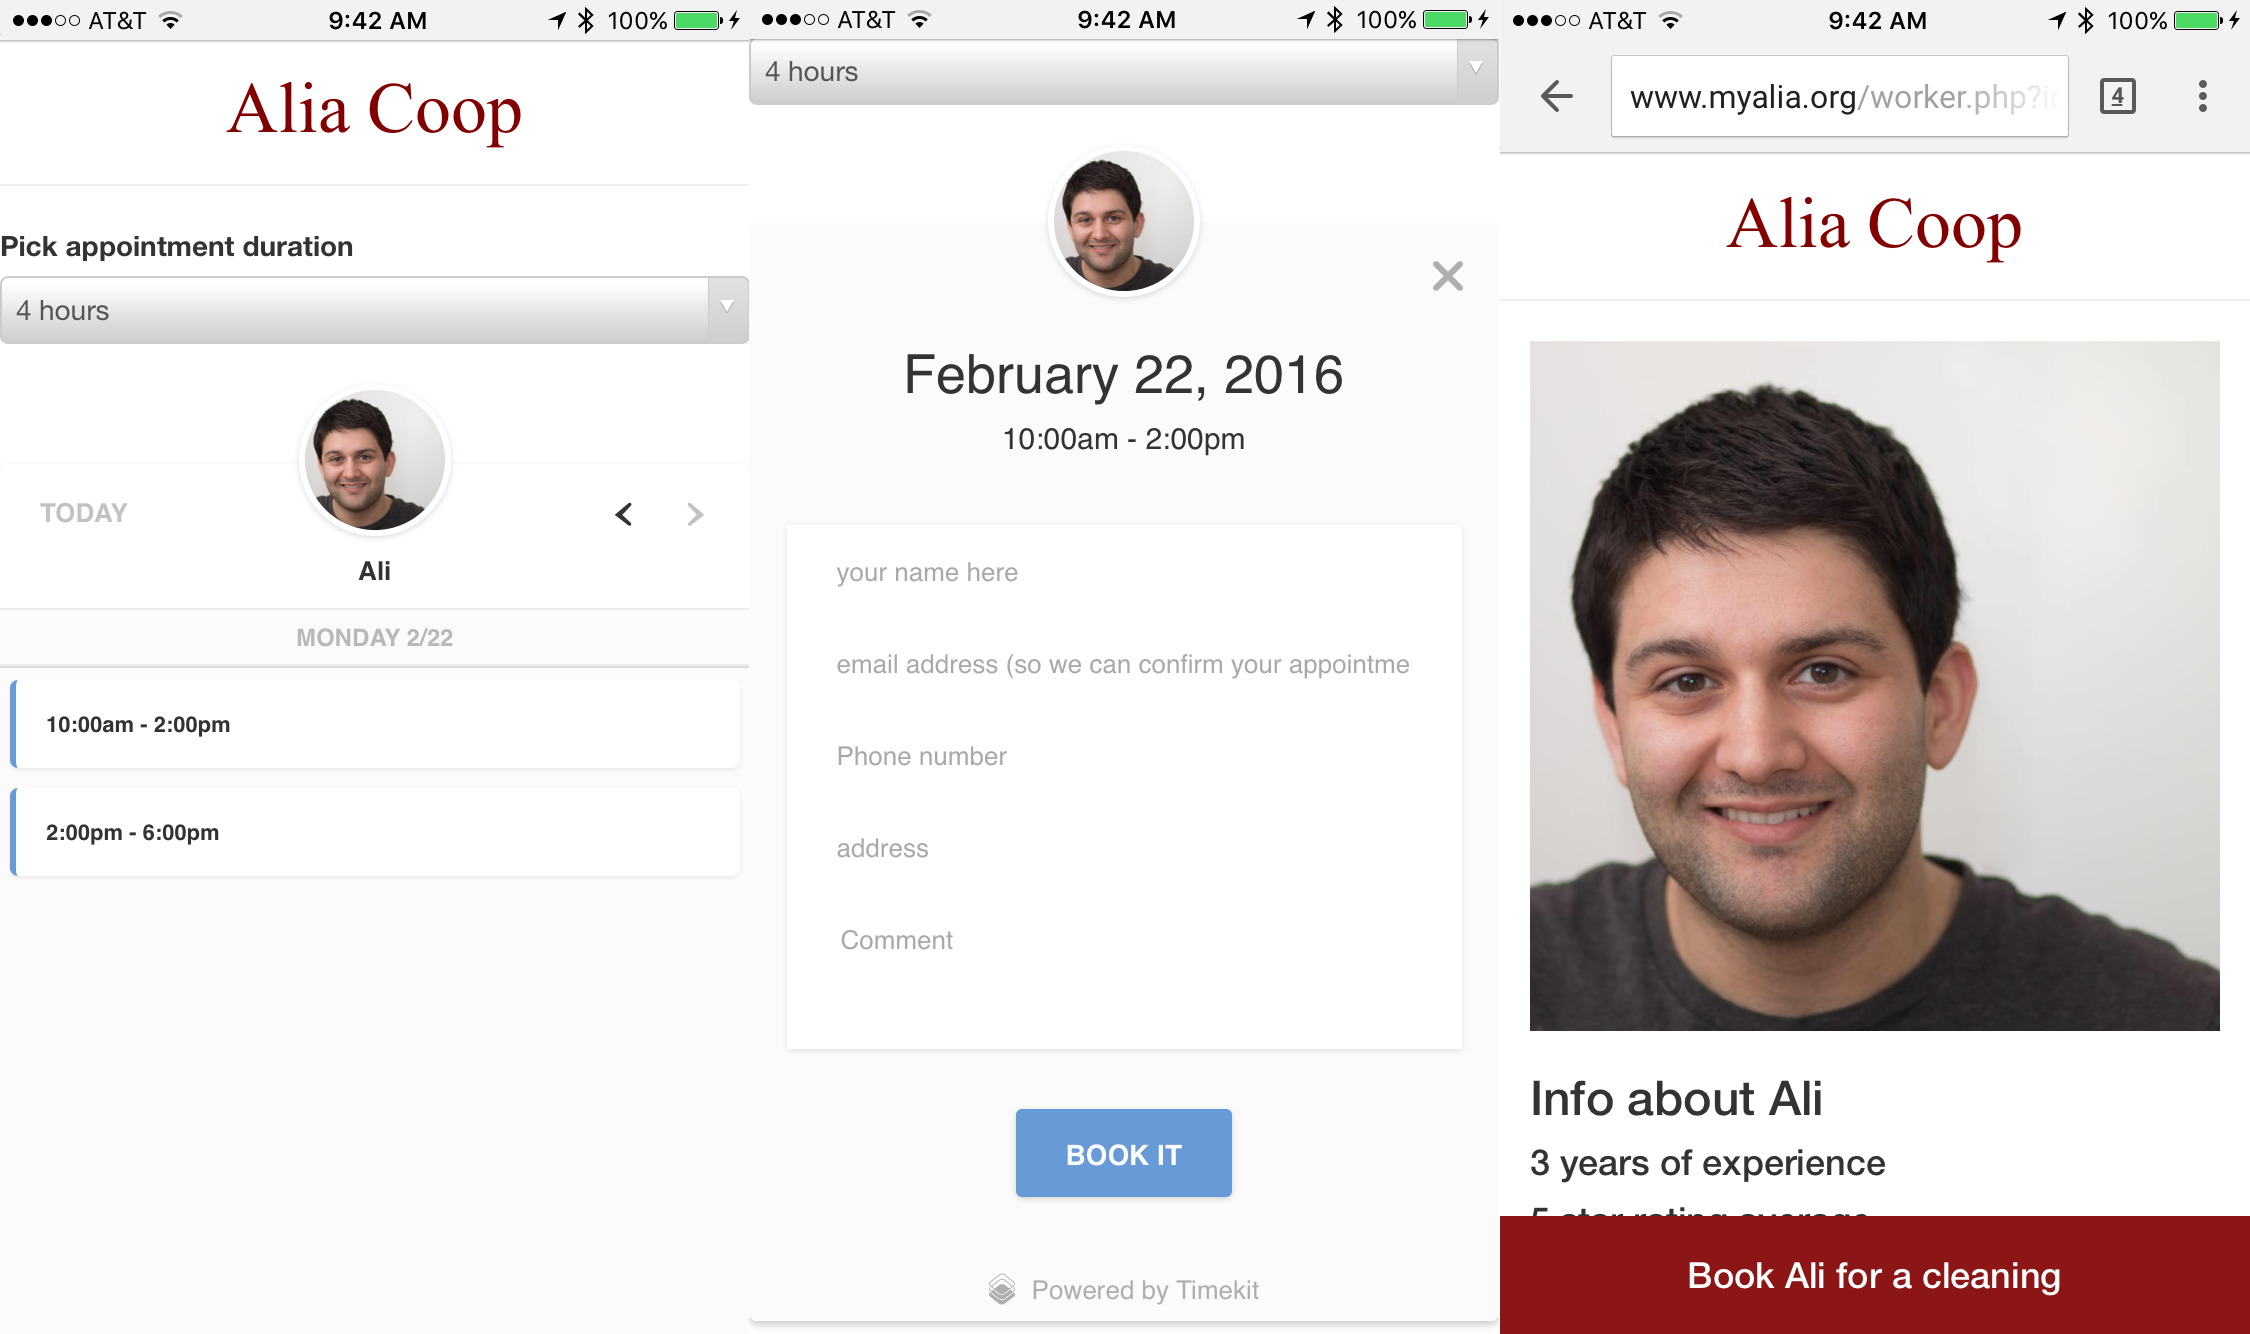
\includegraphics[width=0.7\textwidth]{figures/main.png}
% \end{SCfigure}

The research question that this system asks is:
  how can distributed,
  loosely--affiliated workers
  make effective decisions to govern a cooperative marketplace?
Traditional co--ops operate through scheduled elections to a board and maintain
in--group unity via regular or mandatory meetings.
However,
worker cooperatives at national and international scales could become unwieldy to govern;
empirically,
worker cooperatives become proportionally rarer as one looks to larger and larger companies,
perhaps in part because the governmental challenges either prevent companies from growing to
(or surviving at)
that scale.

Instead of attempting to scale a single cooperative instance,
we propose mechanisms through which local cohorts of workers can `fork' a co--op's guidelines
to create an editable copy, then launch their own co--op.
This new co--op would still operate within the global Alia infrastructure,
allowing the proliferation of many local co--ops that benefit from the single central infrastructure.
Examples of projects like this one already exist
--- Wikipedia’s source code,
maintained by the Wikimedia Foundation,
is available for others to fork and run independently.
Indeed,
instantiations of Wikipedia operating under different administrative policies exist:
Conservapedia,
the Wikia platform, and
others illustrate the potential to fork this originating source code and run parallel communities.

Our second study leverages our access to this cooperatively owned marketplace,
attempting to understand similar dynamics but
focused on those that arise when online pieceworkers
manage and
govern their own labor market.
We seek to understand:
what issues are most contentious for workers to agree on?
How distributed or centralized do they want the platform's governance to be?
When concerns arise similarly to the externally--owned marketplace,
how does the cooperative market deal with them?
We hypothesize that workers will want a loose confederation.
Because workers hold strong self--images as freelancers,
they may be wary of systems tightly regulating their behavior.

Given our privileged access to the platform,
we will engage in a systematic sampling of fifty workers for semi--structured interviews.
We will sample workers randomly from active users of the system,
stratifying at the level of local co--op to ensure that
we capture local variations even if the co--ops in the network are different sizes.
Separately, we will sample workers who were previously active on the platform but have dropped out.
This second sample will be similarly stratified by local co--op within the Alia system.
The first group
--- active co--op workers ---
will give us access to experiences from workers
who have invested time and effort into the future of distributed worker cooperativism.
However, such workers might be self--selecting to be predisposed to such a model.
Thus, we are separately sampling the second group
--- inactive co--op workers ---
to gain insight into those who decided the model did not sufficiently support their needs.

The semi--structured interviews will begin with
a critical incident analysis that asks the worker to recall
a time that their own efforts were supported by the cooperative's decisions.
Example incidents might include when the collective identity helped the worker acquire more work,
or when it helped them engage in arbitration with an unhappy client.
Second, we will seek critical incidents when the worker felt unsupported by the cooperative's decisions.
Example incidents in this case might include
decisions about taxing all cooperative transactions
in order to pay for administrative and server support for the co--op.
We will then ask workers to describe their level of engagement with
the cooperative's governance,
their levels of trust and familiarity with others in the co--op,
and and the kinds of policy issues that they wish the cooperative would engage with.

The interviews are one thrust of a three--pronged mixed methods analysis.
The second thrust is surveys given to platform users, based on the same sampling techniques.
One of the core challenges of gig work is the distributed nature of its workers,
and trust amongst distributed pseudonymous individuals can be low
\citep{rains2007impact}.
Thus, we will utilize survey instruments intended to study internet--specific social capital
\citep{ellison2007benefits}.
In particular, the survey instrument measures
\begin{inlinelist}
  \item bridging social capital,
  which is social capital accumulated between groups of weaker ties and associated with
    risk-taking,
    information diffusion, and
    participation in a group context; and
  \item bonding social capital,
  which is social capital accumulated between stronger ties and
  associated with favors exchanged between close relationships.
\end{inlinelist}
These measures of social capital will help us understand
the levels of trust in the cooperative generally
(bridging social capital) and
with specific individuals in the cooperative
(bonding social capital).

Next, we will engage in a grounded analysis of the platform's forums.
Alia will conduct most of its cooperative decision--making on an online forum.
We will perform an ethnomethodological analysis of forum posts
on Alia to better understand its process for decision making.
We seek to answer:
what techniques do workers use for coalition-building around an online issue,
and how are conflicts resolved?
What percentage of discussion on the forum is dedicated to policy debate,
versus water cooler chatter or mentorship?
What percentage of co-op workers engage in policy debates,
what percentage lurk (read but do not post), and
what percentage do not even log in to follow debates?

Finally, we will perform
a cross--cultural analysis between the current platforms in
Section \ref{ethnography}
and the cooperative platform in
Section \ref{Alia},
comparing the social dynamics that arise in both platforms.
We expect to find that the social mechanisms people adopt to cope with
--- and to navigate ---
cooperatively--designed and
managed marketplaces differ substantially.
Our policy and design goal is
to understand the kinds of worker collectives that can succeed in an online piecework economy, and
to ensure that workers have access to them.



\section{Work Plan and Timeline}
The effort will proceed over two years.
In the first year,
we will perform the qualitative research with workers in order to understand
their platform policy and governance behaviors.
This includes the 100 interviews with information workers on
  Amazon Mechanical Turk and ``gig workers'' on
  Uber,
  Lyft, and
  Handy.
We will analyze the data using a grounded theory approach.
Simultaneously, in the first year,
we design and implement the Alia platform.

In the second year, we will launch Alia,
grow its use locally in the California Bay Area,
and perform fieldwork with Alia workers to understand their relationship with the cooperative.
This includes interviews with fifty workers,
surveys,
and ethnomethodological analysis of the co--op online forums.

A summary of the work plan is below:

% \begin{center}
  \begin{tabular}{|p{0.15\textwidth}|p{0.8\textwidth}|}
    \hline
    % \thead{<Header 1>} & \thead{<Header 2>} \\ %& \thead{<Header 3>} & \thead{<Header 4>} \\ \hline
\textbf{Period} & \textbf{Milestones} \\
\hline
Year one &
\begin{inlinelist}
  \item Fifty interviews with Mechanical Turk workers;
  \item fifty interviews with Uber/Lyft/Handy workers;
  \item implementation of Alia
\end{inlinelist}
\\
\hline
Year two &
\begin{inlinelist}
  \item Launch and grow Alia;
  \item fifty interviews with Alia workers;
  \item survey of Alia workers;
  \item ethnomethodological analysis of Alia forum
\end{inlinelist}
\\
\hline
  \end{tabular}
% \end{center}



\section{Budget Justification}
Our budget asks for support for a graduate student to lead the
  interviews,
  analysis, and
  platform implementation
over the two years.
This student,
  Ali Alkhatib,
holds undergraduate degrees in
  Anthropology and
  Informatics,
and is currently a Computer Science Ph.D. student,
so he has the training required to engage in both activities.
A second graduate student will aid for one quarter each year,
especially with managing the Alia platform.
PIs Levi and Bernstein will support the effort with one month of summer salary each year.



\section{Current and Pending Support}
Bernstein has received an NSF CAREER award (~\$500k) for research on crowdsourcing,
but none of the currently proposed projects were described in that award.
Levi is the PI for CASBS of a grant from the Rockefeller Foundation (\$150k)
to consider the future of work and workers.
This grant supports a working group and essay solicitation/editing but
no research assistants or other support for Levi.
Bernstein and Levi have received internal grant funding from
Stanford's Cyber Initiative (\$100k)
to engage in a social scientific and engineering effort for the future of online work.
That grant is focused on the design and evaluation of
new forms of teams and organizations for crowd workers,
as well as the design and evaluation of new microwork platforms that grant workers stronger reputation signals they can utilize to get hired.
Bernstein and Levi have applied for additional funding from
Stanford's Cyber Initiative for work described in this proposal (\$100k);
review is pending.



\section{Dissemination Strategy}
Our policy and design goal is to understand
the kinds of worker collectives that can succeed
in an online piecework economy,
and to ensure that workers have access to them.
Our research targets will be top--tier venues in human--computer interaction
(e.g., ACM CHI, ACM CSCW)
and political science and sociology
(e.g., APSR, ASR, AJS, AJPS, POP). 

One main outlet for broader dissemination will be as part of
the Future of Work project at CASBS,
which recently published a series of essays in
Pacific Standard and placed op eds in important newspapers and online sources.
The relevant editors remain keen for new and additional material,
and various other magazines
(print and online),
such as American Prospect and Boston Review,
are also interested in possible publication of articles from this project. 

A second set of outlets will be through
the NDWA's relationships with labor advocates and the press.
Our collaborators within the NDWA will manage this effort.
They are eager to position the NDWA and
the NDWA's Fair Care Labs
as an organization working on behalf of the growing class of gig workers.




\section{Conclusion}
An increasing number of workers are re--entering a piecework economy
via online data work and ``gig'' work.
This new online piecework is highly distributed and
individualistic in character, yet
workers still face the same challenges as ever in
representation and
collective behavior.
How are workers reacting to their situation,
and how are they empowered and inhibited in creating collectives
to air grievances and make decisions?
We seek to understand whether the set of online tools that have led to major collective efforts such as Wikipedia and social networks will likewise produce a new set of collective opportunities for workers.

Our work will broadly inform the ongoing policy debates about how to regulate the gig economy.
Gig workers are debated regularly in the pages of major newspapers,
however little literature has deeply investigated their position within the labor force,
how they weave together an income via many small piecework jobs,
and how they organize themselves.
Our goal is to aid this debate by contributing strong empirical evidence of workers' needs and lives under this new piecework economy.






\pagebreak
\begin{appendices}

\section{Social Capital Survey Scale}
These scales are adapted from \citet*{ellison2007benefits}.
Each item is posed as a 7--point Likert scale agree/disagree statement.

\subsection*{Bridging Social Capital Scale}
\begin{itemize}
  \item I feel I am part of the Alia community
  \item I am interested in what goes on at Alia
  \item Alia is a good place to be
  \item I would be willing to contribute money to Alia
  \item Interacting with people at Alia makes me want to try new things
  \item Interacting with people at Alia makes me feel like a part of a larger community
  \item I am willing to spend time to support general Alia activities
  \item In Alia, I come into contact with new people all the time
  \item Interacting with people at Alia reminds me that everyone in the world is connected
\end{itemize}


\subsection*{Bonding Social Capital Scale}
\begin{itemize}
  \item There are several people in Alia I trust to solve my problems
  \item If I needed an emergency loan of \$100, I know someone in Alia I can turn to
  \item There is someone in Alia I can turn to for advice about making very important decisions
  \item If I needed an emergency loan of \$100, I know someone in Alia I can turn to
  \item The people I interact with in Alia would be good job references for me
  \item I do not know people in Alia well enough to get them to do anything important (reversed)
\end{itemize}

\end{appendices}


\pagebreak
\bibliographystyle{plainnat}
\bibliography{references}
\end{document}